	% TODO: Label auf technisches Objekt
	
	\chapter{Entwicklung eines organischen Objekts} 
	%TODO Einleitung: Idee
	% explizite Bezug auf Ultimaker 2, andere Drucker liefern andere Ergebnisse
	% Besonderheiten eines organischen Objekts

	Das Ziel dieser Studienarbeit ist es, zwei unterschiedliche Objekte zu designen und zu drucken. Im vorherigen Kapitel \ref{chapter:techObj} wird die Entwicklung eines technischen Objekts beschrieben. Bei einem technischen Objekt sind die Anspr�che an genaue Bema�ungen hoch, das Objekt selbst sollte so einfach wie m�glich gestaltet sein. Dadurch besteht es oft aus einfachen geometrischen Formen. Allgemein liegt der Fokus auf der Funktionalit�t des Objekts. Um technische Objekte zu designen, wird in der Regel eine \ac{CAD}-Software verwendet. \\
	In diesem Kapitel wird eine andere Art eines Objekts beschrieben: Das organische Objekt. Im Gegensatz zu einem technischen Objekt steht hier nicht die reine Funktionalit�t im Vordergrund. Organische Objekte sind Objekte, die in der Natur vorkommen und nicht k�nstlich vom Menschen gefertigt wurden, beispielsweise Lebewesen oder Pflanzen. In der Regel besitzen diese Objekte kaum Ecken, Kanten oder gerade Fl�chen. \\
	Im Folgenden werden das Design und der Druck eines solchen Objekts beschrieben, im Anschluss folgt ein Fazit �ber die generelle Eignung des Ultimaker 2 f�r den Druck organischer Objekte.
	Wie bereits im vorigen Kapitel bezieht sich diese Arbeit h�ufig auf den Ultimaker 2, der im Kapitel \ref{chapter:techGr:ultimaker2} vorgestellt wird. In der Arbeit mit einem anderen Drucker k�nnen sich Vorgehensweise und Ergebnis deutlich unterscheiden.
	
	

	\section{Konzept}
	\label{chapter:orgObj:konzept}
% --> "Strichm�nnchen"
	Wie zu Beginn des Kapitels beschrieben, soll das organische Objekt runde, gew�lbte Fl�chen aufweisen. F�r diese Studienarbeit wurde ein dreidimensionales Strichm�nnchen als Objekt gew�hlt. Dieses kann unter Verwendung mehrerer Zylinder und Kugeln modelliert werden und enth�lt somit einige gew�lbte Fl�chen. 
	Der Kopf des Strichm�nnchens wird als Kugel modelliert, der restliche K�rper besteht aus sieben Zylindern. Einer davon dient als K�rper und je ein Zylinder wird verwendet, um ein Bein zu modellieren. Die Arme werden mit je zwei Zylinder modelliert. Dadurch kann ein Ellbogengelenk simuliert werden und abwechslungsreiche Armhaltungen werden m�glich.  
	
	
	
	%TODO ist eigenes Kapitel Entwurf n�tig?
	\section{Entwurf}
	% Arbeit mit Blender
	
	\piccaption{Design des organischen Objekts  \label{fig:orgObj:orgObj}}
	\parpic[r]{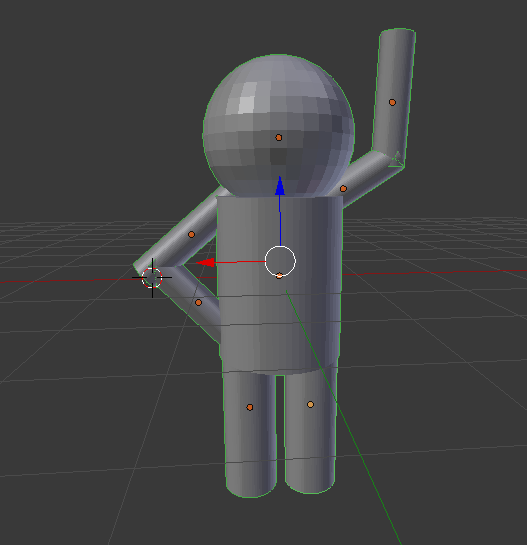
\includegraphics[width=.3\textwidth]{images/orgObj/orgObj}}
	
	
	Das im vorigen Abschnitt beschriebene dreidimensionale Strichm�nnchen wurde mithilfe der Software blender modelliert. Zusammengesetzt ist es aus Zylindern f�r die Arme, Beine und den Rumpf, wie im vorherigen Abschnitt \ref{chapter:orgObj:konzept} beschrieben.
	
	\picskip{0}
	\vspace*{2em}


	
	\newpage
	
	\section{Druck des Objekts}
	% Wie w�re es ideal gewesen?, fertiges Objekt 
	% Welche Parameter? --> spezifisch beim organischen Objekt
	% Verlinkung zu Fehlern
	
	\begin{figure}
		FIGURE NOCH JCIHT DRIN
	\end{figure}
	
	\piccaption{Liegender Druck des organischen Objekts  \label{fig:orgObj:oO_liegend}}
	\parpic[r]{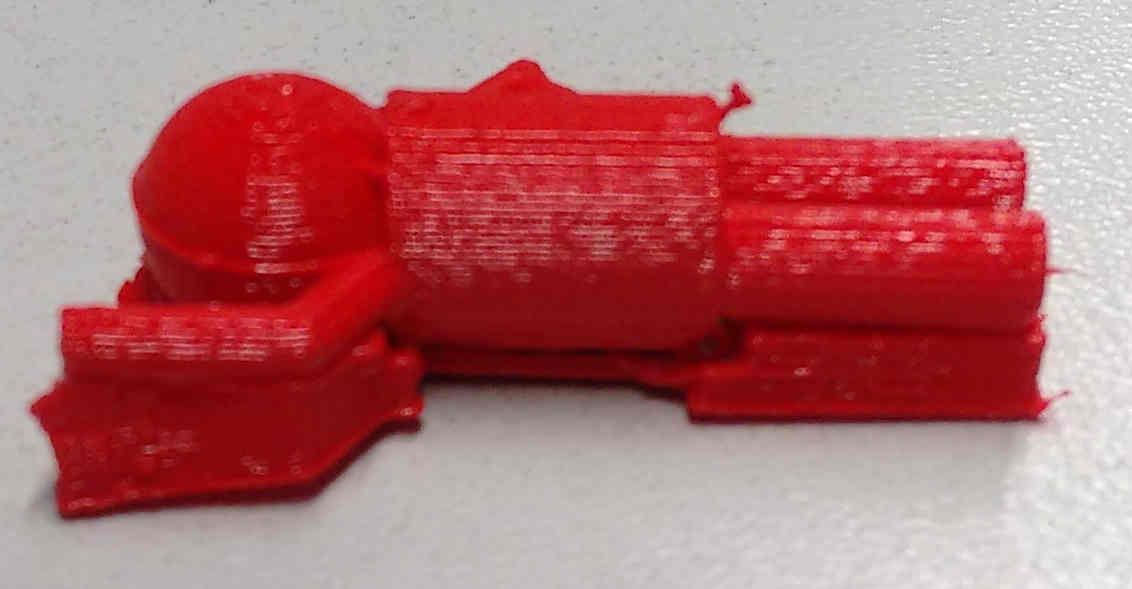
\includegraphics[width=.2\textwidth]{images/orgObj/oO_liegend}}	




	Das Objekt wird in zwei verschiedenen Positionen gedruckt. Einmal wird das M�nnchen liegend auf der Druckplatte positioniert, einmal stehend. 
	Auff�llig ist, dass beim liegenden (?) M�nnchen die Kugel, die den Kopf darstellt, eine starke Kante in der Mitte aufweist. Beim stehenden M�nnchen gelingt die Kugel besser.
	
	\piccaption{Druck des stehenden organischen Objekts  \label{fig:orgObj:oO_stehend}}
	\parpic[r]{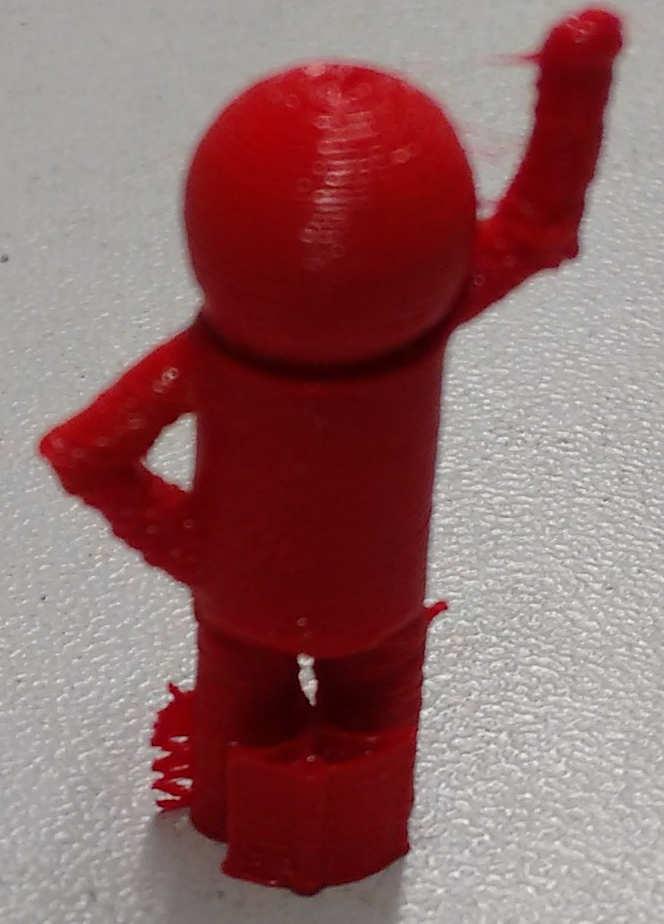
\includegraphics[width=.2\textwidth]{images/orgObj/oO_stehend}}	
	
	\picskip{0}
	
	% \section{Aufgetretene Fehler}\frac{Z�hler}{Nenner}
	% Bilder
	% Fehleranalyse, [Ma�nahmen --> technische Grundlagen]
	
	\section{Fazit: Eignung f�r organische Objekte}
	% bezogen auf Ultimaker
	
	